\documentclass{article}

\usepackage[left=1cm, right=1cm, top=1cm, bottom=2cm]{geometry}
\usepackage{listingsutf8}
\usepackage[utf8]{inputenc}
\usepackage[T1]{fontenc}
\usepackage{xcolor}
\usepackage{amssymb}
\usepackage{stmaryrd}
\usepackage{amsmath}
\usepackage{mathtools}
\usepackage{parskip}
\usepackage{xypic}
\usepackage{tikz}
\usepackage{svg}
\usepackage{pdfpages}
\usepackage{hyperref}
\usepackage{titlesec}
\usepackage[normalem]{ulem}
\usepackage{graphicx}

\usetikzlibrary{shapes.callouts}

\DeclarePairedDelimiter\ceil{\lceil}{\rceil}
\DeclarePairedDelimiter\floor{\lfloor}{\rfloor}

\newcommand{\schem}[3]
{
	\begin{figure}[ht]
		\centering
		\textbf{#1}\par\medskip
		\includegraphics[scale=#3]{figures/figure#2}
		\caption{}
	\end{figure}
}

\lstset{inputencoding=utf8/latin1}

\lstnewenvironment{case}
{
	\renewcommand\lstlistingname{Case}
	\lstset{style = mystyle}
}{}

\newcommand{\code}[1]{\lstinline[style = mystyle]{#1}}

\lstset
{
    frame=tb,
    tabsize=4,
    showstringspaces=false,
    numbers=left,
    commentstyle=\color{gray},
    keywordstyle=\color{blue},
    stringstyle=\color{red},
		literate=
		{á}{{\'a}}1 {é}{{\'e}}1 {í}{{\'i}}1 {ó}{{\'o}}1 {ú}{{\'u}}1
    {Á}{{\'A}}1 {É}{{\'E}}1 {Í}{{\'I}}1 {Ó}{{\'O}}1 {Ú}{{\'U}}1
    {à}{{\`a}}1 {è}{{\`e}}1 {ì}{{\`i}}1 {ò}{{\`o}}1 {ù}{{\`u}}1
    {À}{{\`A}}1 {È}{{\'E}}1 {Ì}{{\`I}}1 {Ò}{{\`O}}1 {Ù}{{\`U}}1
    {ä}{{\"a}}1 {ë}{{\"e}}1 {ï}{{\"i}}1 {ö}{{\"o}}1 {ü}{{\"u}}1
    {Ä}{{\"A}}1 {Ë}{{\"E}}1 {Ï}{{\"I}}1 {Ö}{{\"O}}1 {Ü}{{\"U}}1
    {â}{{\^a}}1 {ê}{{\^e}}1 {î}{{\^i}}1 {ô}{{\^o}}1 {û}{{\^u}}1
    {Â}{{\^A}}1 {Ê}{{\^E}}1 {Î}{{\^I}}1 {Ô}{{\^O}}1 {Û}{{\^U}}1
    {œ}{{\oe}}1 {Œ}{{\OE}}1 {æ}{{\ae}}1 {Æ}{{\AE}}1 {ß}{{\ss}}1
    {ç}{{\c c}}1 {Ç}{{\c C}}1 {ø}{{\o}}1 {å}{{\r a}}1 {Å}{{\r A}}1
    {€}{{\EUR}}1 {£}{{\pounds}}1
}

\lstdefinestyle{mystyle}
{
    language = Caml,
		otherkeywords = {ref,;,decr,incr,false,true,raise,when,log,failwith,sin,cos,tan,mod,abs,exp,sqrt,tanh,int_of_float,float_of_int,int_of_float,unit,char_of_int,int_of_char},
}

\setcounter{secnumdepth}{5}

\titleformat{\paragraph}
{\normalfont\normalsize\bfseries}{\theparagraph}{1em}{}
\titlespacing*{\paragraph}
{0pt}{3.25ex plus 1ex minus .2ex}{1.5ex plus .2ex}

\begin{document}

	\obeylines

	\title{\vspace{-1.7cm}Option informatique: Devoir maison (Noël)\\
	\large Benjamin LOISON (MP*)
			\\24 décembre 2019}
	\date{}
	\maketitle

	\vspace{-2.3cm}\noindent\makebox[\linewidth]{\rule{\paperwidth}{0.4pt}}
	\vspace{4cm}\noindent\makebox[\linewidth]{\rule{\paperwidth}{0.4pt}}
		
		\section{}
			
			\begin{case}
let rec insere l e = match l with
| [] -> [e]
| t::q when e > t -> t::(insere q e)
| t::q when e <> t -> e::l
| t::q -> l;;
			\end{case}
			
		\section{}
		
			La fonction \code{insere} est linéaire en la taille de la liste $l$.
		
		\section{}
		
			\begin{case}
let voisins g s =
	let l = ref [] in
	let rec aux aMaj = match aMaj with
	| [] -> ()
	| t::q -> if t.a = s then l := insere !l t.b
			 else if t.b = s then l := insere !l t.a;
			 aux q;
	in aux g.aMaj;
	!l;;
			\end{case}
		
		\section{}
		
			Sur le graphe $Gex2$, on trouve:
		
			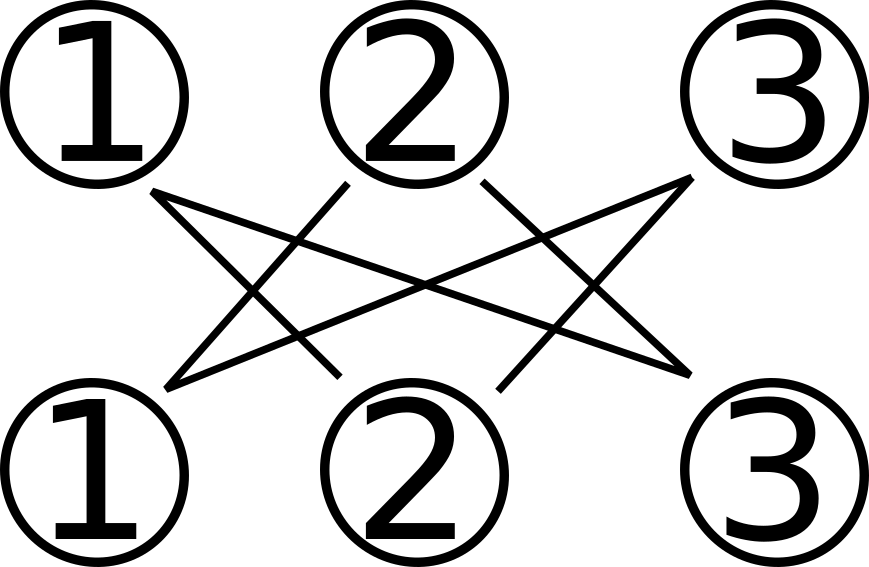
\includegraphics[scale=0.1]{IMG/PNG/4a.png}

			Oui, il y a une bonne coloration de $Gex2$ avec moins de couleurs:

			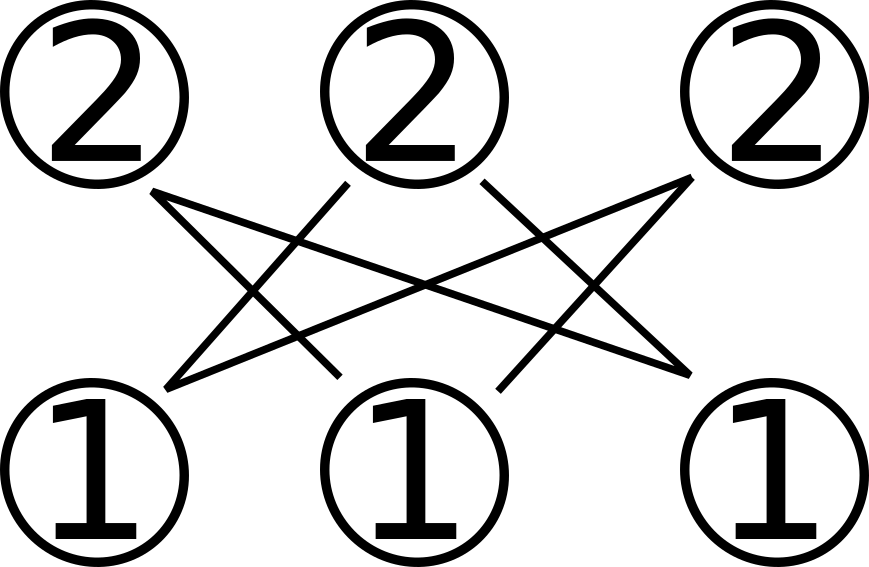
\includegraphics[scale=0.1]{IMG/PNG/4b.png}
			
		\section{}
			
			\begin{case}
let coloration g =
	let t = Array.make g.n 0 in
	for i = 0 to (g.n - 1) do
		let v = voisins g i in
			 let rec aux v b = match v with
			 | [] -> b
			 | a::q when t.(a) = 0 -> b
			 | a::q when t.(a) < b -> aux q b
			 | a::q -> aux q (t.(a) + 1)
			 in t.(i) <- aux v 1;
	done;
	t;;
			\end{case}
		
		\section{}
		
			Pour l'existence, il existe forcément nbc($G$), tel que fc($G$, nbc($G$)) $\neq 0$, par exemple:
	on a fc($G$, n($G$)) $\neq 0$ d'où l'existence et on a directement $\forall p \geq$ nbc($G$), fc($G$, $p$) $\neq 0$
	est != 0 car cela revient par récurrence à ne pas utiliser la nouvelle couleure

	Pour l'unicité, on procède par l'absurde, supposons l'existence de nbc($G$) et nbc'($G$)
	distincts, on a alors clairement min(nbc($G$), nbc'($G$)) qui
	n'appartient pas à EC($G$): contradiction.
		
		\section{}
		
			S'il n'y a aucune arrête, alors tous les sommets peuvent avoir la même coloration donc nbc($G$) = 1.
	
	Ayant le choix du nombre pour la coloration pour chaque sommet parmi $\llbracket 1; n \rrbracket$, on a donc fc($G$, $p$) = $p^{n(G)}$

		\section{}
		
			Tous les sommets sont reliés à tous les autres:
on a donc nbc($G$) = n($G$) et fc($G$, $p$) %TODO

		\section{}
		
			On a clairement nbc($Gex1$) >= 3, on a égalité dans la relation précédente car en considérant les 3 sommets 0, 3 et 4, on remarque qu'étant tous liés un sommet doit être distinct de ces 2 voisins donc il faut au moins 3 couleurs.
			
			
		
		\section{}
		
			\begin{case}
let prem_voisin g s =
	List.hd (voisins g s);;
			\end{case}
			
		\section{}
		
			\begin{case}
let prem_ni g =
	let i = ref 0 and b = ref 0 in
	while !i < (g.n - 1) do
		if (List.length (voisins g !i)) <> 0 then (b := !i; i := g.n);
		incr i
	done;
	!b;;
			\end{case}
		
		\section{}
		
			\begin{case}
let h g =
	let s1 = prem_ni g in
	let s2 = prem_voisin g s1 in
	let rec aux l = match l with
	| [] -> []
	| t::q when (t.a = s1 && t.b = s2) || (t.b = s1 && t.a = s2) -> aux q
	| t::q -> t::(aux q)
	in {n = g.n; aMaj = aux g.aMaj};;
			\end{case}
			
		\section{}
		
			\begin{case}
let k g =
	let s1 = prem_ni g in
	let s2 = prem_voisin g s1 and hg = h g in
	let chg i = if i = s2 then s1 else (if i > s2 then i - 1 else i) in
	let rec aux l = match l with
	| [] -> []
	| t::q -> {a = chg t.a; b = chg t.b}::(aux q)
	in {n = g.n - 1; aMaj = aux hg.aMaj};;
			\end{case}
			
		\section{}
		
			
			
		\section{}
		
			
			
		\section{}
		
			
			
		\section{}
		
			
			
		\section{}
		
			\begin{case}
let difference p q = (* TO KNOW: does array or list are like pointers in argument - only array are mutable (sure ?) *)
	let r = Array.copy p in
	for i = 0 to (Array.length q) - 1 do
		r.(i) <- r.(i) - q.(i)
	done;
	r;;
			\end{case}
			
		\section{}
		
			\begin{case}

			\end{case}
			
		\section{}
		
			\begin{case}
let eval p x =
	let n = Array.length p in
	let res = ref p.(n - 1) in
	for i = 2 to n do
		res := x * (!res) + p.(n - i)
	done;
	!res;;
			\end{case}
			
		\section{}
		
			\begin{case}

			\end{case}
		
\end{document}
